\documentclass{standalone}
\usepackage{tikz}
\usetikzlibrary{positioning,shapes,snakes}
\begin{document}
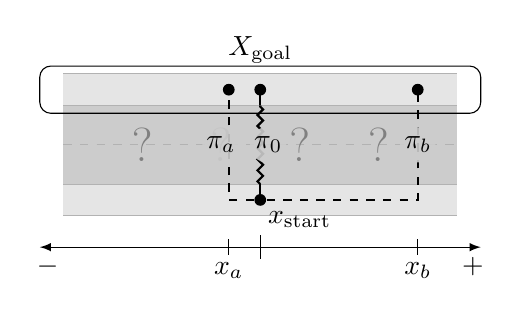
\begin{tikzpicture}

   \tikzset{>=latex} % arrow heads

   \fill[black!10] (-2.5, 0.5) rectangle (2.5, 0.9);
   \fill[black!20] (-2.5,-0.5) rectangle (2.5, 0.5);
   \fill[black!10] (-2.5,-0.9) rectangle (2.5,-0.5);
   \draw[black!30]
      % horizontal lines
      (-2.5,-0.9) -- (2.5,-0.9)
      (-2.5,-0.5) -- (2.5,-0.5)
      (-2.5, 0.5) -- (2.5, 0.5)
      (-2.5, 0.9) -- (2.5, 0.9);
      % upper sidewalk lines
      %(-2.25, 0.9) -- (-2.25, 0.5)
      %(-1.75, 0.9) -- (-1.75, 0.5)
      %(-1.25, 0.9) -- (-1.25, 0.5)
      %(-0.75, 0.9) -- (-0.75, 0.5)
      %(-0.25, 0.9) -- (-0.25, 0.5)
      %( 0.25, 0.9) -- ( 0.25, 0.5)
      %( 0.75, 0.9) -- ( 0.75, 0.5)
      %( 1.25, 0.9) -- ( 1.25, 0.5)
      %( 1.75, 0.9) -- ( 1.75, 0.5)
      %( 2.25, 0.9) -- ( 2.25, 0.5)
      % lower sidewalk lines
      %(-2.25,-0.9) -- (-2.25,-0.5)
      %(-1.75,-0.9) -- (-1.75,-0.5)
      %(-1.25,-0.9) -- (-1.25,-0.5)
      %(-0.75,-0.9) -- (-0.75,-0.5)
      %(-0.25,-0.9) -- (-0.25,-0.5)
      %( 0.25,-0.9) -- ( 0.25,-0.5)
      %( 0.75,-0.9) -- ( 0.75,-0.5)
      %( 1.25,-0.9) -- ( 1.25,-0.5)
      %( 1.75,-0.9) -- ( 1.75,-0.5)
      %( 2.25,-0.9) -- ( 2.25,-0.5);
   % middle line and question marks
   \draw[black!30,dashed] (-2.5,0) -- (2.5,0);
   \node[black!50] at (-1.5,0) {\LARGE ?};
   \node[black!50] at (-0.5,0) {\LARGE ?};
   \node[black!50] at ( 0.5,0) {\LARGE ?};
   \node[black!50] at ( 1.5,0) {\LARGE ?};
   
   \node[fill=black,circle,inner sep=1.5pt] (xstart) at (0,-0.7) {};
   \node at (0.5,-0.95) {$x_{\mbox{\scriptsize start}}$};
   
   \draw[black,<->] (-2.8,-1.3) -- (2.8,-1.3);
   \draw[black] (0,-1.15) -- (0,-1.45);
   \node at (-2.7,-1.55) {$-$};
   \node at ( 2.7,-1.55) {$+$};
   
   \draw[color=black,rounded corners]
      (-2.8,0.4) rectangle (2.8,1.0);
   \node at (0,1.2) {$X_{\mbox{\scriptsize goal}}$};
   
   % first solution
   \draw[color=black,thick,
      snake=zigzag,segment length=4pt,segment amplitude=1pt]
      (0,-0.5) -- (0,0.5);
   \draw[color=black,thick] (0,-0.7) -- (0,-0.5) (0,0.5) -- (0,0.7);
   \node[fill=black,circle,inner sep=1.5pt] at (0,0.7) {};
   \node[circle,inner sep=0.5pt,fill=black!20,opacity=0.9,text opacity=1]
      at (0.1,0) {$\pi_0$};
   
   % left solution
   \draw[color=black,thick,dashed] (xstart) -- (-0.4,-0.7) -- (-0.4,0.7);
   \node[fill=black,circle,inner sep=1.5pt] at (-0.4,0.7) {};
   \node[circle,inner sep=0.5pt,fill=black!20,opacity=0.9,text opacity=1]
      at (-0.5,0) {$\pi_a$};
   \draw[black] (-0.4,-1.2) -- (-0.4,-1.4);
   \node at (-0.4,-1.6) {$x_a$};
   
   % right solution
   \draw[color=black,thick,dashed] (xstart) -- (2,-0.7) -- (2,0.7);
   \node[fill=black,circle,inner sep=1.5pt] at (2,0.7) {};
   \node[circle,inner sep=0.5pt,fill=black!20,opacity=0.9,text opacity=1]
      at (2,0) {$\pi_b$};
   \draw[black] (2,-1.2) -- (2,-1.4);
   \node at (2,-1.6) {$x_b$};

\end{tikzpicture}%
\end{document}
